\chapter{Ewaluacja}

\subsection{Odometria}
Robot korzysta z nawigacji zliczeniowej w celu połączenia pomiarów odległości zebranych z otoczenia i aproksymacji ich położenia na płaszczyźnie względem jednego ustalonego punktu. Zliczaniu podlegają dwie wartości - dystans przejechany wzdłuż oraz obrót pojazdu w miejscu.Rys. \ref{fig:odom-axis-simplified} przedstawia rzeczywisty oraz uproszczony model budowy robota, obrazujący jego sposób poruszania się. Zamiast uwzględniać obie osi i 4 koła, upraszcza się go do formy robota o jednej osi, z jedną parą kół. Gdy oba koła poruszają się w tę samą stronę, robot przesuwa się w przód lub w tył. Gdy pracują przeciwbieżnie - obraca się.

\begin{figure}[ht]
	\centering
		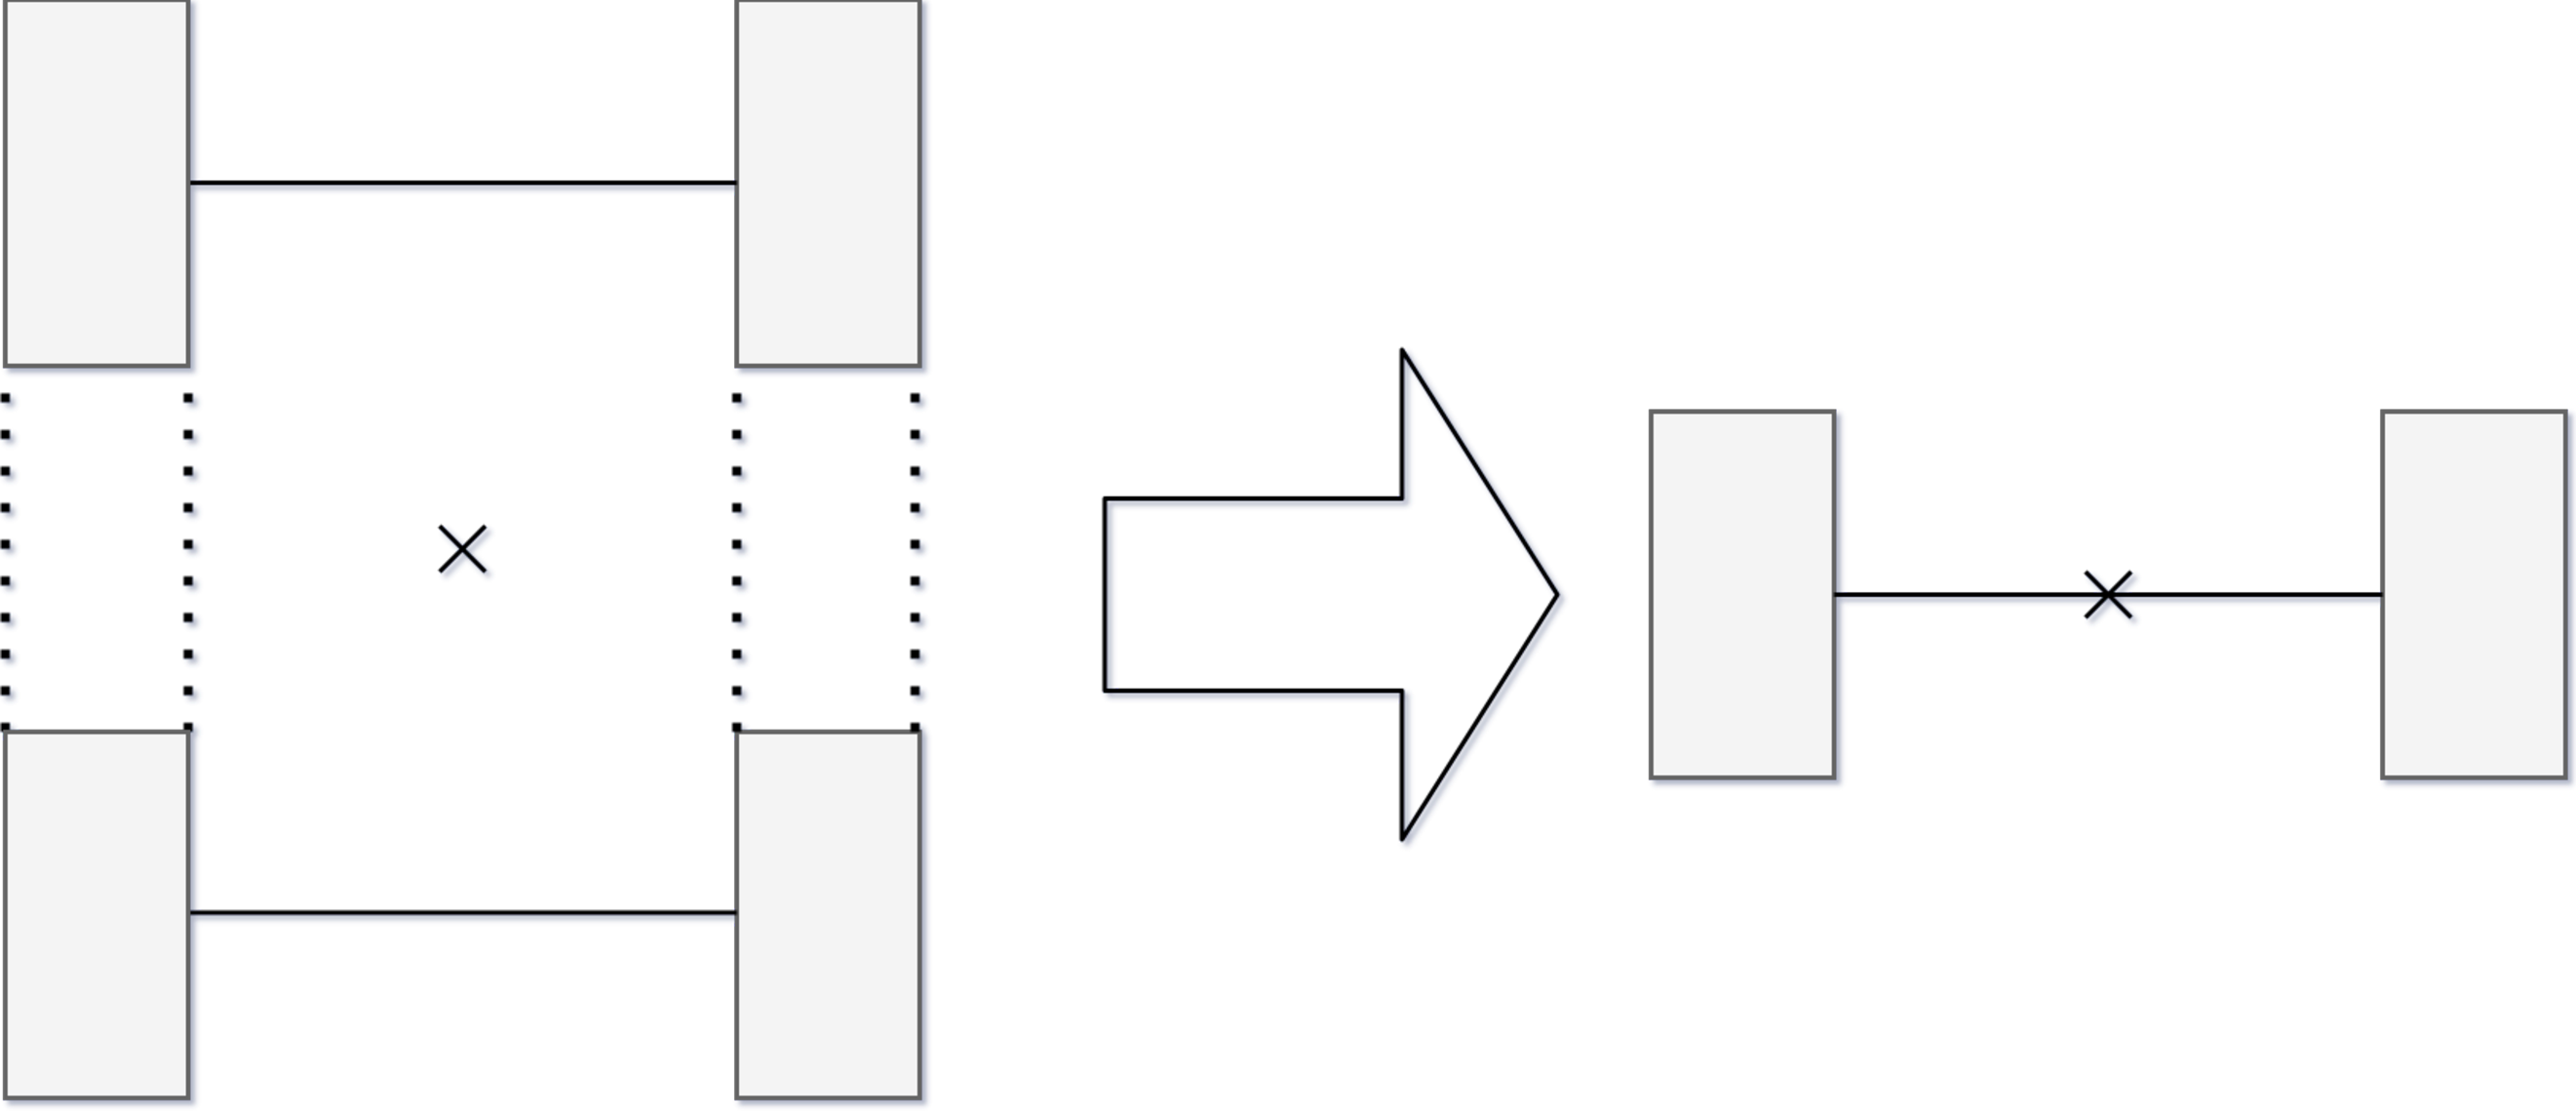
\includegraphics[width=0.8\linewidth]{rys/robot-odometry-simplified.pdf}
	\caption{Model rzeczywisty i uproszczony}
	\label{fig:odom-axis-simplified}
\end{figure}


Pierwszym pomysłem było wykorzystanie enkoderów do pomiaru translacji pojazdu wzdłuż jego osi ruchu, pozostawiając zliczanie obrotu funkcjom korzystającym z magnetometru.

>TODO obrazek z zaznaczonym placementem enkoderów w robocie

Enkodery zostały zamontowane w miejscu przedstawionym na Rys. >TODO. Napęd podany od serwa przez zębatkę przenosi napęd zarówno na koło jak i enkoder z przekładniami 1:1 w obu przypadkach. Dzięki takiemu rozwiązaniu pełny obrót enkodera odpowiada pełnemu obrotowi koła. Enkoder obrotowy EC-11 generuje 20 impulsów przy kącie obrotu 360°. Należy obliczyć stosunek ilości impulsów do przejechanego dystansu. Wiedząc ile impulsów generuje enkoder, oraz znając wymiary koła w łatwy sposób można to obliczyć.

%>TODO dodać obliczenia
%>TODO dać te podpisy
%DPR - Distance to Pulse Ratio
%r - promień koła
%p - liczba impulsów na obrót
%przejechany dystans=DPR*p
%srednica kola 50mm=5cm 2*pi*2,5=15,7cm na obrot
%20ppr
\begin{equation}
    DPR = \frac{2 \pi r}{p}
\end{equation}

Znając współczynnik DPR aby obliczyć przejechany dystans wystarczy zmierzyć ilość impulsów jakie wystąpiły podczas przejazdu a następnie pomnożyć je przez DPR. Otrzymany wynik oznacza przesunięcie robota wyrażone w centymetrach. Jako że platforma posiada dwa enkodery, a nie jest możliwe zachowanie idealnie prostego toru jazdy, wyciągana jest średnia liczba impulsów. Ze względu na grubość oraz wypustki na gąsienicach efektywny dystans przejechany będzie większy. Dla kompensacji tej różnicy wartość DPR została skorygowana ręcznie do takiej, przy której błąd przemieszczenia robota zawierał się w granicy 10cm na zadany dystans 100cm. Poniższy listing prezentuje funkcję realizującą to zadanie.

\begin{lstlisting}[basicstyle=\footnotesize\ttfamily]
//MOVE
case 9:
{
    reset_encoders();
    float val = getArgument(command, 1).toInt() * 1.325;

    if (val > 0)
        driveMotors(90, 90);
    else
        driveMotors(-90, -90);

    val = abs(val);
    while ((left_encoder_counter + right_encoder_counter) / 2 < val)
    {
    }

    driveMotors(0, 0);
    delay(100);
    Serial2.println("OK");
}
\end{lstlisting}

Podczas wykonywania polecenia \emph{MOVE} zadawana jest pełna prędkość na gąsienice i w pętli sprawdzana jest średnia ilość impulsów wygenerowanych przez enkoder. W parametrze polecenia został przekazany dystans do przejechania - w momencie w którym średnia ilość impulsów przekroczy jego wartość, serwa zostają zatrzymane.
\\ 

Obrót (funkcja \emph{ROTATE}) polega na zadaniu przeciwstawnych wartości prędkości na obie gąsienice. W celu obrotu poruszają się one przeciwbieżnie, z równymi prędkościami. Pierwsza implementacja funkcji obrotu przebiega jak następuje:
\\

Na początku mierzony jest azymut początkowy i obliczany jest azymut końcowy (początkowy + wartość obrotu). Dalej wykonywana jest ta sama funkcja co w przypadku \emph{ROTATE\_TO} przyjmująca parametr azymutu końcowego. Podczas obrotu, w pętli, sprawdzana jest różnica kąta aktualnego od zadanego. Jeżeli wartość bezwzględna obrotu znajdzie się w zakresie ±10° robot zatrzyma się.

\begin{lstlisting}[basicstyle=\footnotesize\ttfamily]
void rotateTo(int azimuth)
{
    if (calcAngleDistance(getAzimuth(), azimuth) > 0)
        driveMotors(-90, 90);
    else
        driveMotors(90, -90);

    while (true)
    {
        if (abs(calcAngleDistance(getAzimuth(), azimuth)) <= 10)
            break;
        delay(10);
    }
    driveMotors(0, 0);
    delay(100);
}
\end{lstlisting}

Takie rozwiązanie jest dobre, o ile magnetometr jest skalibrowany i funkcjonuje poprawnie. Niestety, podczas skanów okazało się że nie można polegać na pomiarach z tego sensora - więcej o tym znajduje się w sekcji \ref{sec:mag_cal}. Z tego powodu koniecznym okazała się zmiana podejścia do pomiaru obrotu.

Poniższy listing przedstawia nowe podejście. Jest ono mniej dokładne od poprzedniego, bardziej podatne na dryf (błąd obrotu kumuluje się), natomiast taki pomiar jest odporny na zakłócenia pola magnetycznego.
Tym razem pomiar jest analogiczny jak w przypadku ewaluacji polecenia \emph{MOVE}. W pętli również sprawdzana jest średnia wartość bezwzględna dystansu przejechanego przez gąsienice, jednak tym razem poruszają się one przeciwbieżnie. Ilość zliczonych impulsów należy przemnożyć przez pewien współczynnik tak aby odpowiadały one kątowi obrotu. Platforma kończy ruch w momencie gdy średnia wartość przekroczy obliczony próg obrotu.

Tym razem współczynnik został wyznaczony eksperymentalnie. Najpierw przyjęto wartość 1. Następnie zadawany był kąt obrotu 90°, po czym mierzony był rzeczywisty kąt obrotu. Jeżeli wynosił on więcej, współczynnik redukowano o 0,1; analogicznie gdy obrót był mniejszy niż zadano. Gdy tak zgrubna regulacja była niewystarczająca (albo za mały albo za duży obrót), krok został zmniejszony do 0,05. Po kolejnej zmianie kroku do 0,02 czynność powtarzano do momentu w którym dalsza korekcja nie była konieczna.

Taka implementacja obrotu została zachowana do końca projektu.

\begin{lstlisting}[basicstyle=\footnotesize\ttfamily]
// ROTATE
    case 11:
    {
        reset_encoders();
        float val = getArgument(command, 1).toInt() * 0.164;
        if (val > 0)
            driveMotors(-90, 90);
        else
            driveMotors(90, -90);

        val = abs(val);
        while ((left_encoder_counter + right_encoder_counter) / 2 < val)
        {
        }

        delay(100);
        driveMotors(0, 0);
        Serial2.println("OK");
    }
    break;
\end{lstlisting}

\subsubsection{Kalibracja magnetometru}
\label{sec:mag_cal}

%>TODO powiedz o tym jak sie skaszaniło przy przewodzie pod podłogą
%>TODO koniecznie daj screenshoty
%opisz hard i soft iron offset
%wspomnij o potrzebie zastosowania filtru (np kalmana)



%% 3d rozkalibrowany
\begin{figure}[ht]
	\centering
		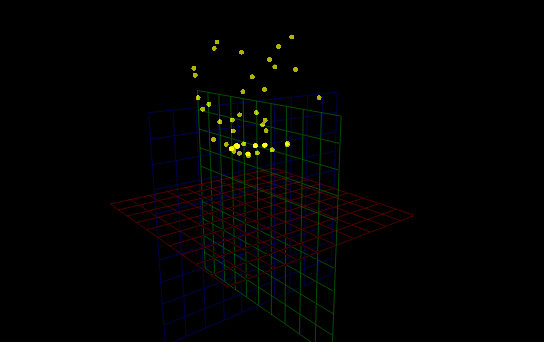
\includegraphics[width=0.8\linewidth]{rys/ScanBot-03-magnetometer-3d-decalibrated.PNG}
	\caption{>TODO}
	\label{fig:xxx}
\end{figure}

% %% 3d kalibracja hard 1
% \begin{figure}[ht]
% 	\centering
% 		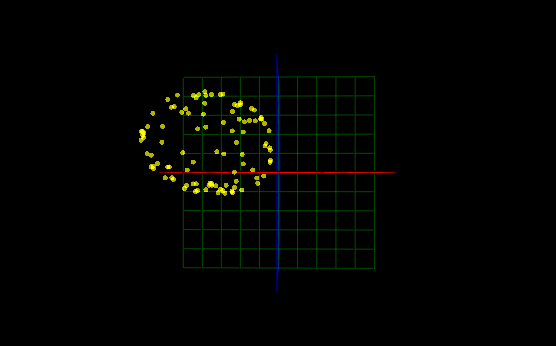
\includegraphics[width=0.8\linewidth]{rys/ScanBot-04-magnetometer-3d-calibration.PNG}
% 	\caption{>TODO}
% 	\label{fig:xxx}
% \end{figure}

% %% 3d kalibracja hard 2
% \begin{figure}[ht]
% 	\centering
% 		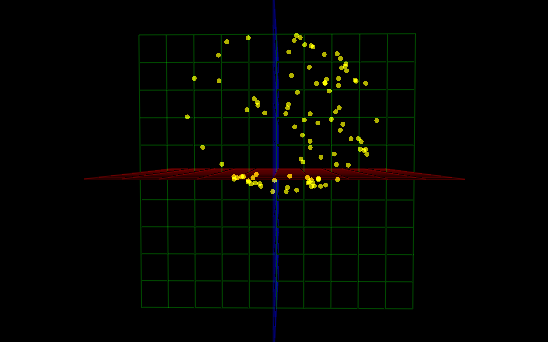
\includegraphics[width=0.8\linewidth]{rys/ScanBot-05-magnetometer-3d-calibration.PNG}
% 	\caption{>TODO}
% 	\label{fig:xxx}
% \end{figure}

% %%3d kalibracja hard 3
% \begin{figure}[ht]
% 	\centering
% 		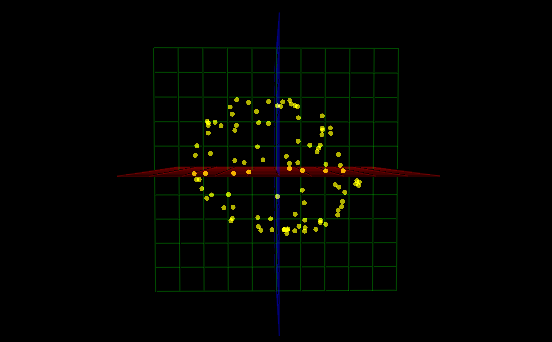
\includegraphics[width=0.8\linewidth]{rys/ScanBot-06-magnetometer-3d-calibration.PNG}
% 	\caption{>TODO}
% 	\label{fig:xxx}
% \end{figure}

%>TODO mozna opisac proby zmapowania jajka na kolko

%%2d rozkalibrowany
\begin{figure}[ht]
	\centering
		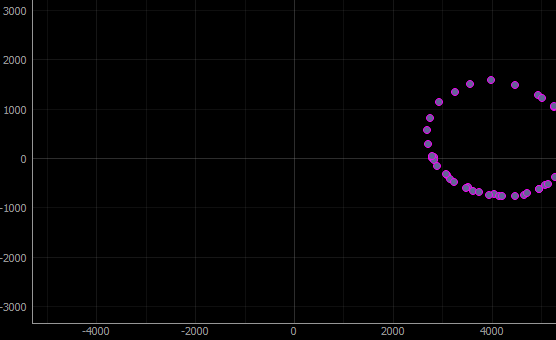
\includegraphics[width=0.8\linewidth]{rys/ScanBot-08-2d-calibration-theta-sigma.PNG}
	\caption{>TODO}
	\label{fig:xxx}
\end{figure}

%2d kalibracja hard
\begin{figure}[ht]
	\centering
		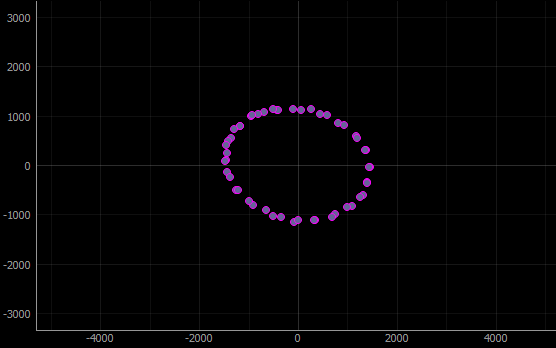
\includegraphics[width=0.8\linewidth]{rys/ScanBot-10-2d-calibration-theta-sigma-2-added-hard-offset-reset-data-so-soft-iron-values-are-proper.PNG}
	\caption{>TODO}
	\label{fig:xxx}
\end{figure}

%2d kalibracja soft
\begin{figure}[ht]
	\centering
		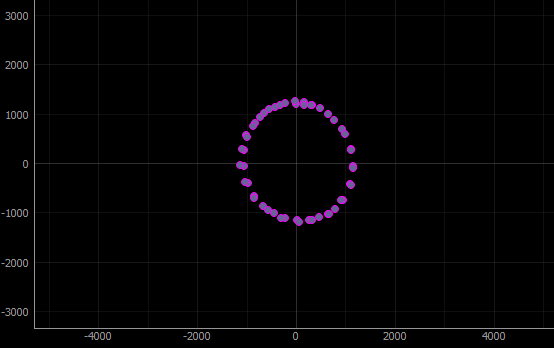
\includegraphics[width=0.8\linewidth]{rys/ScanBot-11-2d-set-theta-then-sigma-and-done.PNG}
	\caption{>TODO}
	\label{fig:xxx}
\end{figure}


% widok finalnego panelu kalibracji
\begin{figure}[ht]
	\centering
		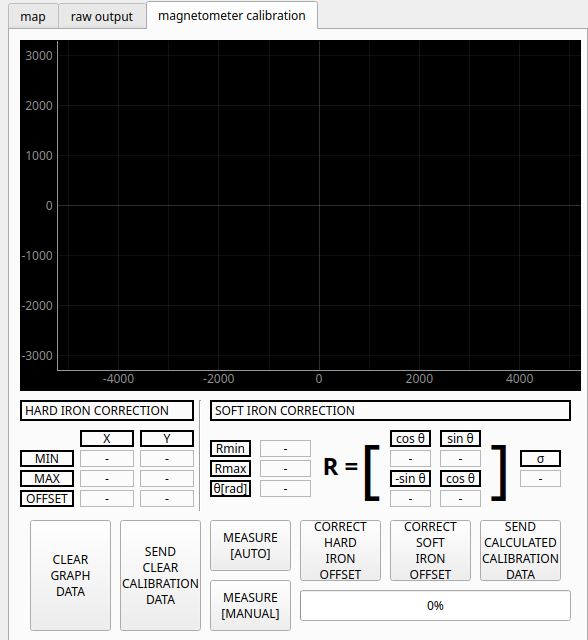
\includegraphics[width=1\linewidth]{rys/main-app-view-magnetom.PNG}
	\caption{Widok sekcji kalibracji magnetometru okna głównego aplikacji}
	\label{fig:main-app-mag-section}
\end{figure}




\begin{figure}[ht]
	\centering
		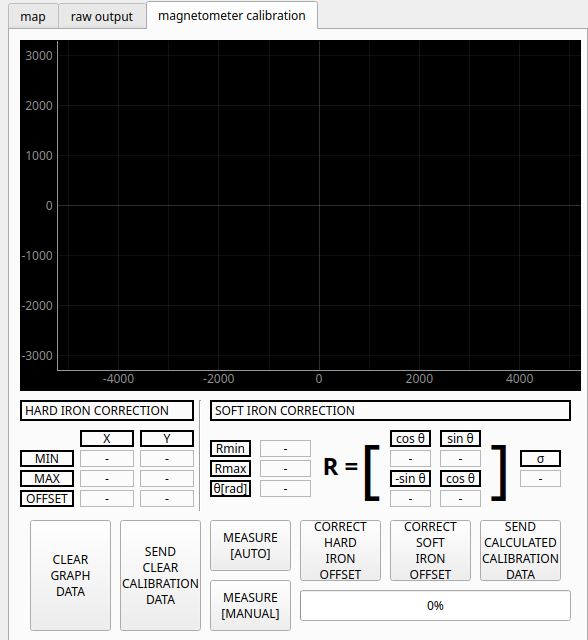
\includegraphics[width=1\linewidth]{rys/main-app-view-magnetom.PNG}
	\caption{Widok sekcji kalibracji magnetometru}
	\label{fig:main-app-mag-section}
\end{figure}


%%przewod - interferencja
\begin{figure}[ht]
	\centering
		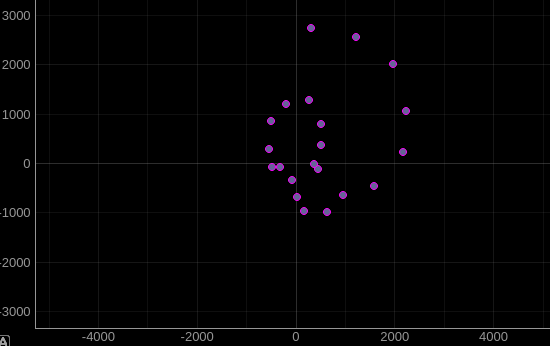
\includegraphics[width=0.8\linewidth]{rys/calibrated-mag-high-interference-broken-rotation.PNG}
	\caption{>TODO}
	\label{fig:xxx}
\end{figure}

%% znowu przewod
\begin{figure}[ht]
	\centering
		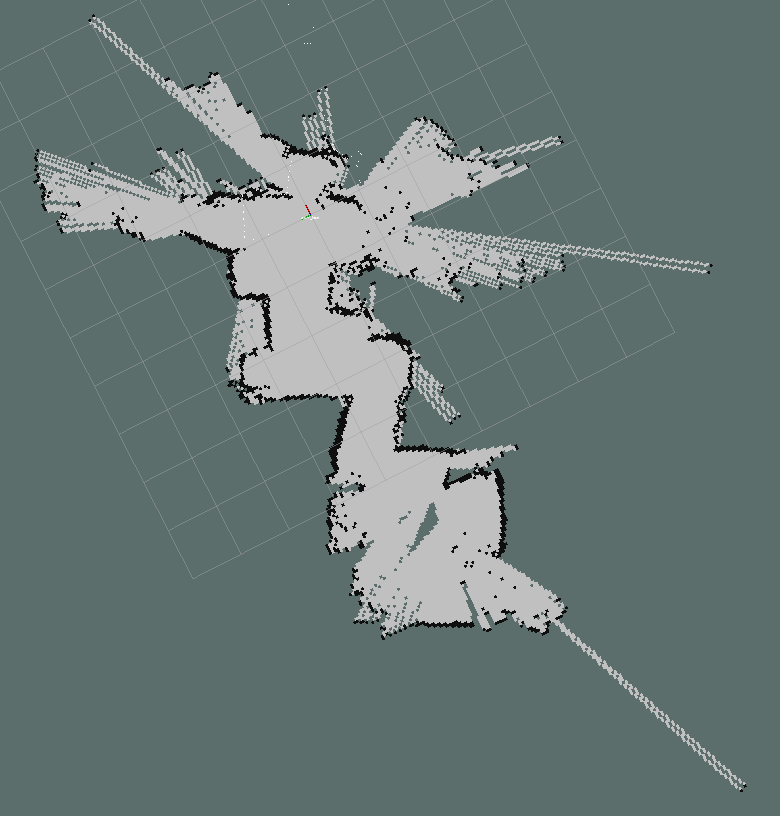
\includegraphics[width=0.8\linewidth]{rys/2020-11-04-170347_1920x1080_scrot.PNG}
	\caption{>TODO}
	\label{fig:xxx}
\end{figure}




\subsubsection{Filtr Kalmana}
\label{sec:kalman}



\subsection{Skan otoczenia i budowa mapy}
Samo zebranie pomiarów i przedstawienie ich w formie czytelnej dla człowieka nie jest trudne w realizacji. Pozyskane dane można przedstawić na wykresie, punkty połączyć prostymi liniami. Problem zaczyna się z agregacją wielu pomiarów, i na tym będzie koncentrował się ten rozdział.

Mając do dyspozycji sensory


%>TODO tu napisac o bazowym mapowaniu pkt na plaszczyzne
%o swojej implementacji ze scorem
%nastepnie o tym co moznaby dalej (translacja korekta)
%ale nie zostalo zrobione bo bylo slabe i to wymaga filtrow czasteczek
%i ze jest cos takiego jak cartographer od googla
%ale zdecydowano ze gmapper jest spoko i czemu nie gmapper


\begin{figure}[ht]
	\centering
		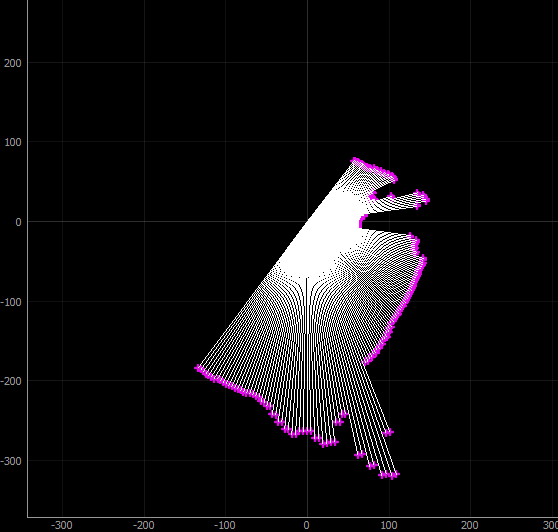
\includegraphics[width=0.5\linewidth]{rys/ScanBot-12-calibrated-room-map1.PNG}
	\caption{>TODO}
	\label{fig:xxx}
\end{figure}

\begin{figure}[ht]
	\centering
		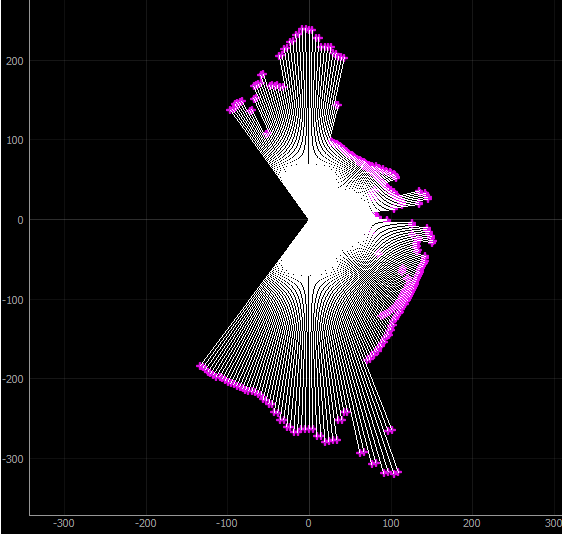
\includegraphics[width=0.5\linewidth]{rys/ScanBot-12-calibrated-room-map2.PNG}
	\caption{>TODO}
	\label{fig:xxx}
\end{figure}

\begin{figure}[ht]
	\centering
		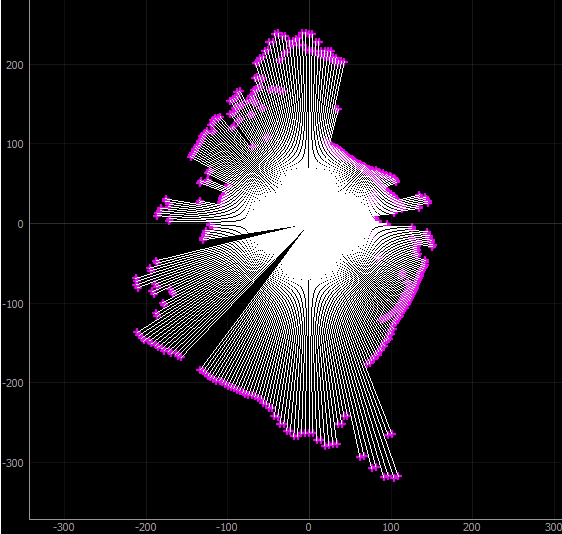
\includegraphics[width=0.5\linewidth]{rys/ScanBot-12-calibrated-room-map3.PNG}
	\caption{>TODO}
	\label{fig:xxx}
\end{figure}

\begin{figure}[ht]
	\centering
		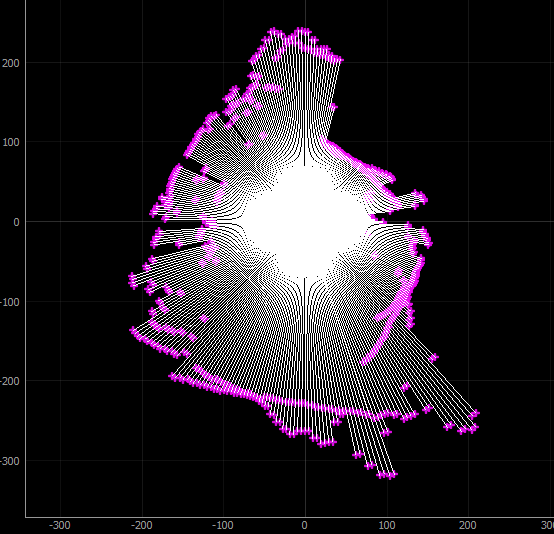
\includegraphics[width=0.5\linewidth]{rys/ScanBot-12-calibrated-room-map4.PNG}
	\caption{>TODO}
	\label{fig:xxx}
\end{figure}


\subsubsection{UMBenchmark\cite{Borenstein1995}}
%>TODO tu dac fotki koniecznie
%jakies rysunki nabazgrane z kwadratami
% i powiedziec ze sie nie pokrywalo najlepiej
% dac tabelke z pozycjami
% pokazac obliczenia center of gravity itd
% wyszlo ~1proc czyli to bez sensu
% wiec robot juz jezdzi wystarczajaco dobrze

% >TODO nawiaz do wczesniej wspomnianych rzeczy
% powiedz co po kolei jak sie zmieniało
% z czym były problemy
% o tutaj mala podpowiedz:

% sensor dzwieku jest do kitu za duza fluktuacja pluz ogromny kąt plus za duzy blad pomiaru plus za dlugi pomiar
% sharp mniejszy kąt mniejsza fluktuacja krotki pomiar ale podatnosc na swiatlo
% lidar super miodzio
% serwo kiepskie i wibruje/zacina się co powoduje błędy na krawędziach
% magnetometr-biblioteka koryguje jedynie hard iron i jest do kitu
% ze wzgledu na moc obliczeniowa najlepiej bylo samemu zaimplementowac soft i hard iron
% zeby bylo prosciej tylko 2 wymiary, niestety nie kompensujemy tiltu. ale i tak zalozenie jest ze jezdzimy po plaskim

% używanie arcsin zamiast atan2 z ifami podowowało błąd że correction czasem obracał elipsę nie w tę stronę